\documentclass[12pt,a4paper]{article}

% for polish language
\usepackage{polski}

% for some math symbols
\usepackage{amssymb}

% correct footnotes placement
\usepackage[bottom]{footmisc}

% for \say command
\usepackage{dirtytalk}

% change title of the bibliography
\def\bibname{Referencje}\let\refname\bibname

% for advanced math formulas
\usepackage{mathtools}

\usepackage{listings}

% links
\usepackage{hyperref}
% \hypersetup{
%     colorlinks,
%     citecolor=black,
%     filecolor=black,
%     linkcolor=black,
%     urlcolor=blue
% }

% image displaying
\usepackage{subcaption}
\usepackage{graphicx}

\usepackage{multirow} 
\usepackage{makecell}

\title{Dokumentacja do projektu z USD}

\author{Roman Moskalenko \and Pavel Tarashkevich}
\date{}

\begin{document}

\maketitle

\section{Treść zadania}

\textbf{LL1.AnyTrading Stocks}\\

Zapoznaj się z \href{https://github.com/AminHP/gym-anytrading}{gym-anytrading} oraz
zbiorem danych tam dostępnym:

LL1 - STOCKS\_GOOGL

Przygotuj agenta podejmującego akcje na rynku i uczącego się ze wzmocnieniem
oraz porównaj jego skuteczność ze strategią losową. Przetestuj co najmniej 2 różne
algorytmy uczenia ze wzmocnieniem. Przygotuj skrypt umożliwiający wizualizację
działań wytrenowanego agenta.

\section{Projekt wstępny}

\subsection{Założenia ogólne}

Dla zaimplementowania agenta zajmującego się handlowaniem na rynku mamy
posłużyć algorytmem uczenia się ze wzmocnieniem (dalej RL). Jako założenie przyjmujemy,
że środowisko agenta, którym posłużymy się, będzie tylko częściowo odwzorowywać
rzeczywiste środowisko rynku. Będzie ono zawierało minimalny zestaw
atrybutów, niezbędnych do nauczenia agenta oraz najprostsze akcje
(\emph{kup}/\emph{sprzedaj}) do dyspozycji agenta.

Zakładamy, że algorytmy RL sprawdzą się lepiej, niż strategia losowa.

\subsection{Krótki opis przydzielonego środowiska}

W ramach projektu będziemy używać środowiska do symulacji handlowania
na rynku akcji podane w treści zadania: \href{https://github.com/AminHP/gym-anytrading}{gym-anytrading}.
Dane środowisko jest pochodną popularnego środowiska do trenowania agentów
RL \href{https://github.com/openai/gym}{gym} i zawiera ono podstawowe
jego funkcje. Zawiera ono także minimalny zestaw atrybutów opisujących
rynek akcji. Ono zawiera specjalną instancję \mbox{\emph{StockEnv}},
która naszym zdaniem najlepiej odwzorowuje środowisko dla naszego
zadania.

\subsection{Wybrane algorytmy}

Do realizacji zadania wybraliśmy algorytmy A2C, PPO. Literatura dotycząca
stosowania algorytmów RL dla trenowania agentów do handlowania na rynku
akcji wskazuje, że te dwa algorytmy dobrze się sprawdzają
\cite{ensemble_strat}.

Algorytm A2C (\emph{Advantage Actor-Critic}) bazuje na pomyśle
wykorzystania sieci neuronowych do aproksymacji polityki agenta (aktor)
oraz do aproksymacji funkcji wartości (krytyk).

Algorytm PPO (\emph{Proximal Policy Optimization}) rozwija algorytm A2C,
wykorzystując specjalne metody do optymalizacji polityki agenta.

\medskip

Porównamy je z algorytmem losowym.

\subsection{Biblioteki wybrane do realizacji projektu}

\begin{itemize}
  \item \textbf{gym-anytrading} - środowisko do trenowania agentów RL do
        handlowania na rynku akcji.
  \item \textbf{\href{https://github.com/notadamking/Stock-Trading-Visualization}{Stock-Trading-Visualization}} -
        skrypt do wizualizacji działań agenta oparty o bibliotekę \emph{matplotlib}.
  \item \textbf{\href{https://github.com/DLR-RM/stable-baselines3}{stable-baselines}} -
        biblioteka zawierająca gotowe implementację algorytmów RL.
\end{itemize}

\subsection{Propozycja eksperymentów do przeprowadzenia}\label{exps_proposal}

Zamierzamy przeprowadzić trenowanie wybranych modeli stosując różne
podejścia wyboru podzbioru danych uczących - danych z różnych okresów
czasowych.

Nie jest oczywiste jak powinna wyglądać strategia nagradzania agenta:
warto uwzględnić ten fakt, że w handlowaniu na rynku może być większa
preferencja natychmiastowego zysku, aby móc go potem wykorzystać w
późniejszych akcjach agenta. Uwzględnimy to, dostosowując parametr
dyskontowania nagród.

\label{metrics}
W celu ewaluacji działania algorytmów zastosujemy następujące metryki
m.i. wykorzystane w \cite{ensemble_strat}: \emph{Cumulative return},
\emph{Annualized return}, \emph{Annualized volatility}, \emph{Sharpe ratio},
\emph{Max drawdown}.

\pagebreak
\section{Projekt końcowy}

\subsection{Uzupełnienie projektu wstępnego}

Niestety postanowiliśmy zrezygnować z korzystania ze skryptów \textbf{Stock-Trading-Visualization},
ponieważ opierają się na innej bibliotece do handlowania na rynku przez
agentów RL i jest niekompatybilny z \textbf{gym-anytrading}.

W przykładach użycia biblioteki \textbf{gym-anytrading} zauważyliśmy
użycie biblioteki
\textbf{\href{https://github.com/ranaroussi/quantstats}{quantstats}}
do analizy operacji finansowych. Postanowiliśmy ją wykorzystać, gdyż
pozwala wyznaczyć metryki wspomniane przez nas w rozdziale
\ref{exps_proposal}.

\subsection{Opis środowiska gym-anytrading}

Aby mieć możliwość poprawnie interpretować wyniki uczenia i działania
modeli na danym środowisku musieliśmy zagłębić się w jego strukturę.
Chcielibyśmy wymienić kilka najważniejszych cech, które zwróciły naszą
uwagę:

\begin{itemize}
  \item \textbf{pozycje \emph{Long} i \emph{Short}} -
        W zarysie: w pozycji \emph{Long} agent chcę kupować akcje, kiedy
        ceny na nie są niskie, żeby w przyszłości zyskać na wzroście cen,
        a w pozycji \emph{Short} agent chcę sprzedawać akcje, kiedy ceny
        są wysokie, aby potem na uzyskane środki kupić akcje kiedy ceny
        zmaleją, zyskując na różnicy.
  \item \textbf{nagrody (reward)} - różnica pomiędzy ceną zamknięcia akcji w danej
        chwili a ceną zamknięcia akcji w chwili ostatniej transakcji
        (transakcja jest wykonywana w sytuacji kiedy agent miał pozycję
        \emph{Long} oraz wybrał akcję \emph{Sell}).
  \item \textbf{zysk (profit)} - jest aktualizowany wraz z każdą
        transakcją, a jest równy liczbie akcji, które posiadaliśmy podczas
        ostatniej transakcji, razy aktualna cena zamknięcia akcji.

\end{itemize}

\pagebreak
\subsection{Uczenie agentów}

Dane dostępne z biblioteki \textbf{gym-anytrading}, które zostały wykorzystane
w ramach projektu podzieliliśmy na dwa podzbiory: dane uczące i dane testowe.
Podział został dokonany w taki sposób, że pierwsze $80\%$ danych tworzą
zbiór uczący, a reszta - zbiór testowy. \\

Z powodów oczywistych agent wykorzystujący politykę losową nie był uczony.
\smallskip

Wybraliśmy domyślne konfiguracje algorytmów A2C i PPO.
Ich uczenie dokonywano w ciągu 1,000,000 kroków,
gdzie za krok uznajemy pojedynczą akcją dokonaną przez
agenta na danym środowisku. Uczenie przeprowadziliśmy dla różnych zestawów
parametrów \emph{rozmiaru okna} - zdarzeń historycznych dostępnych agentowi
w każdym kroku działania (10, 20, 30) oraz \emph{dyskonta} (0.7, 0.9, 0.99).

Po przetestowaniu nauczonych agentów uznaliśmy, że ich sprawność nie
jest satysfakcjonująca, dlatego też użyliśmy rekurencyjnej wersji
algorytmu PPO (dla \emph{rozmiaru okna} 30 oraz \emph{dyskonta} 0.99), którą
pobraliśmy z repozytorium \href{https://github.com/Stable-Baselines-Team/stable-baselines3-contrib/pull/53}
{stable-baselines3-contrib} (ze względu na brak oficjalnej implementacji
w bibliotece stable-baselines3).

Uczenie jest dokonane łącznie 3 razy
dla każdego algorytmu w celu zmniejszenia wpływu
losowości na uzyskane wyniki.

Na rysunku \ref{fig:training} pokazano przebieg uczenia agentów.
Jak widać sumy nagród uzyskiwane przez agentów dla parametru dyskonta
równego 0.7 są wyraźnie mniejsze w porównaniu z 0.9 i 0.99. Także widać, że
rozmiar okna czasowego nie wiele zmienia pod względem efektywności uczenia.
Charakterystycznym jest ten fakt, że algorytm PPO pokazuje lepszą wydajność,
niż A2C, czego można było po nim się spodziewać. Nieco dziwnym jest ten
fakt, że sumy nagród uzyskiwane przez algorytm rekurencyjny PPO są mniejsze
od sum nagród uzyskiwanych przez algorytm domyślny.

\begin{figure}[!ht]
  \centering
  \includegraphics[width=0.8\textwidth]{../src/plot0.pdf}
  \caption{Przebieg uczenia agentów w przeciągu 1,000,000 kroków.
    Na wykresie pokazano zakres sum nagród, uzyskany przez
    średnią sumę nagród oraz odchylenia standardowego.}
  \label{fig:training}
\end{figure}

\pagebreak
\subsection{Ewaluacja działania agentów}

Do ewaluacji działania nauczonych agentów każdy z nich przetestowaliśmy
na danych testowych, wykorzystane metryki z rodziału \ref{metrics}
uzyskaliśmy za pomocą raportów Quantstats. Wyniki wybranego zbioru
nauczonych agentów podajemy w tabeli \ref{tab:results}.

Krótki opis tych metryk podany poniżej:

\begin{itemize}
  \item \textbf{Cumulative return} - zwrot inwestycji na całym okresie czasowym.
  \item \textbf{Annualized return} - zwrot inwestycji w okresie jednego roku.
  \item \textbf{Annualized volatility} - miara rozrzutu zwrotów uzyskanych w
        okresie jednego roku, najczęściej liczona jako odchylenie standardowe
        zwrotów.
  \item \textbf{Sharpe ratio} - stosunek różnicy średniego zwrotu i
        stopy wolnej od ryzyka (w naszym projekcie przyjęliśmy ją równą 0)
        do wartości \emph{volatility}. \emph{Sharpe ratio} większe od 1
        zwykle uznawane jest za dobre \cite{sharpe}.
  \item \textbf{Max drawdown} - największa wartość różnicy między
        szczytem a kolejnym dołkiem wyrażonej w procentach.
\end{itemize}

\begin{table}[!h]
  \hspace*{-1cm}\begin{tabular}{llllll}
    \hline
    \multicolumn{1}{c}{} & \multicolumn{1}{c}{Cum. return} & \multicolumn{1}{c}{Ann. return} & \multicolumn{1}{c}{Ann. volatility} & \multicolumn{1}{c}{Sharpe ratio} & \multicolumn{1}{c}{Max drawdown} \\
    \hline
    Random               & -71.67\%                        & -49.87\%                        & 15.0\%                              & -4.79                            & -72.23\%                         \\
    A2C                  & -68.82\%                        & -45.36\%                        & 13.14\%                             & -5.06                            & -68.96\%                         \\
    PPO                  & \phantom{-}0.74\%               & -0.75\%                         & 14.71\%                             & \phantom{-}0.1                   & -17.72\%                         \\
    RecPPO               & \phantom{-}14.86\%              & -0.42\%                         & 19.33\%                             & \phantom{-}0.51                  & -23.42\%                         \\
    \hline
  \end{tabular}
  \caption{Wartości metryk sprawności agentów dla danych testowych}
  \label{tab:results}
\end{table}

Wyniki te w postaci bardziej szczegółowej można znaleźć w dodatku \ref{app:reports}.

\medskip

Jak można było się spodziewać agent losowy zachowuje się najgorzej i
nie przynosi żadnego zysku przez cały okres testowy. Algorytm A2C
sprawuje się podobnie do algorytmu losowego, jego działanie nie możemy
uznać za sensowne. Algorytmy z rodziny PPO pokazują o wiele lepsze
wyniki, przy czym modyfikacja o rekurencyjną politykę wyraźnie wzmocniła
algorytm i zwiększyła jego efektywność. Jest to naturalne, gdyż
rozważany w ramach projektu problem jest w uproszczeniu działaniem
na szeregach czasowych, gdzie modele rekurencyjne generalnie dobrze się
sprawują.

Wyniki te są mało satysfakcjonujące, gdyż generalnie algorytmy częściej
tracą, niż zyskują, pomijając fakt, że prawdziwe środowiska do
tradingu są zdecydowanie bardziej złożone.
Stosowanie rekurencyjnej polityki jest mocno zalecane.


\pagebreak
\begin{thebibliography}{9}
  \bibitem{ensemble_strat}
  Yang, Hongyang and Liu, Xiao-Yang and Zhong, Shan and Walid, Anwar,
  Deep Reinforcement Learning for Automated Stock Trading: An Ensemble
  Strategy (September 11, 2020). Available at SSRN:
  \href{https://ssrn.com/abstract=3690996}{https://ssrn.com/abstract=3690996}
  or \href{http://dx.doi.org/10.2139/ssrn.3690996}{http://dx.doi.org/10.2139/ssrn.3690996}
  \bibitem{sharpe}  \url{https://www.investopedia.com/terms/s/sharperatio.asp}
\end{thebibliography}

\pagebreak
\appendix
\section{Raporty Quantstats \\
  dla rozmiaru okna 30 oraz dyskonta 0.99}\label{app:reports}

\begin{figure}[ht!]
  \centering
  \begin{subfigure}[ht!]{0.45\textwidth}
    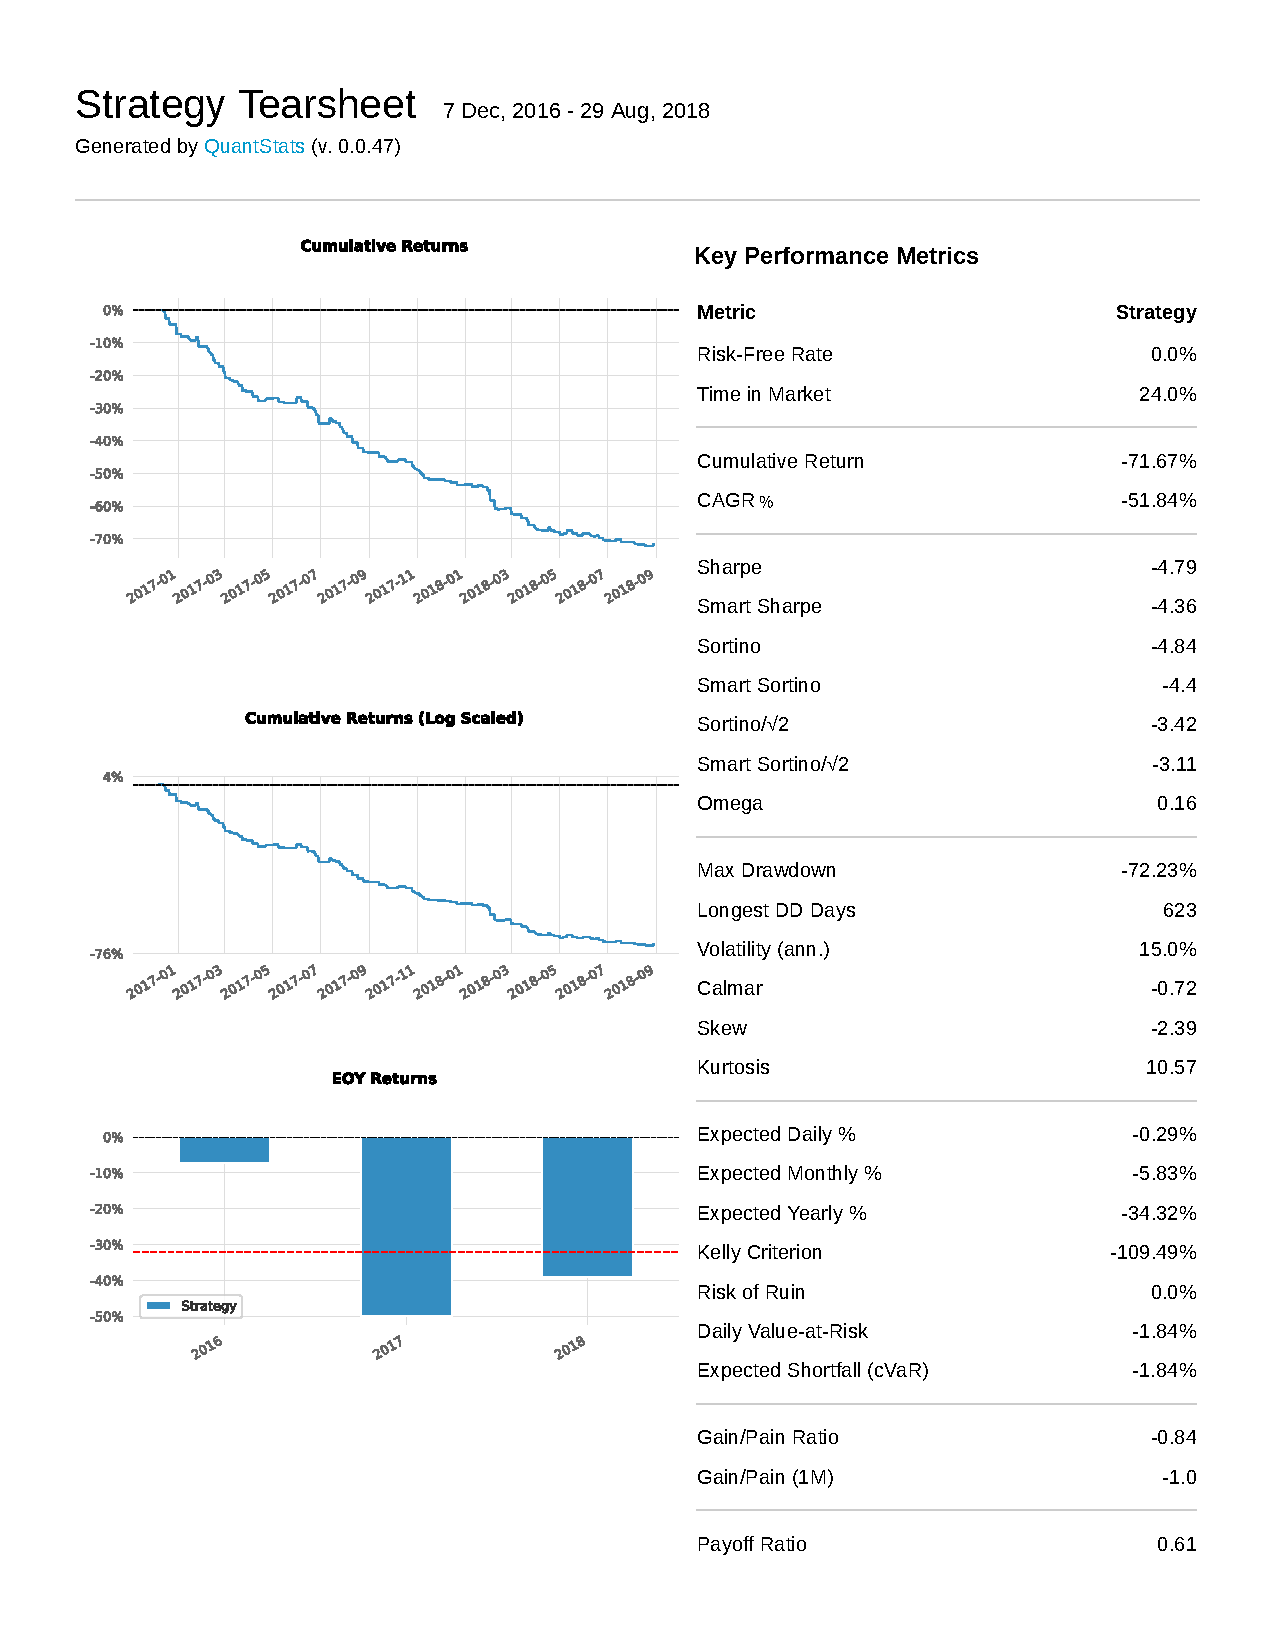
\includegraphics[width=\textwidth]{plots/qs_rand.pdf}
  \end{subfigure}
  \hspace{0.05\textwidth}
  \begin{subfigure}[ht!]{0.45\textwidth}
    \includegraphics[page=2, width=\textwidth]{plots/qs_rand.pdf}
  \end{subfigure}
  \begin{subfigure}[ht!]{0.45\textwidth}
    \includegraphics[page=3, width=\textwidth]{plots/qs_rand.pdf}
  \end{subfigure}
  \caption{Raport Quantstats dla algorytmu losowego na
    danych testowych}
\end{figure}

\begin{figure}[ht!]
  \centering
  \begin{subfigure}[ht!]{0.45\textwidth}
    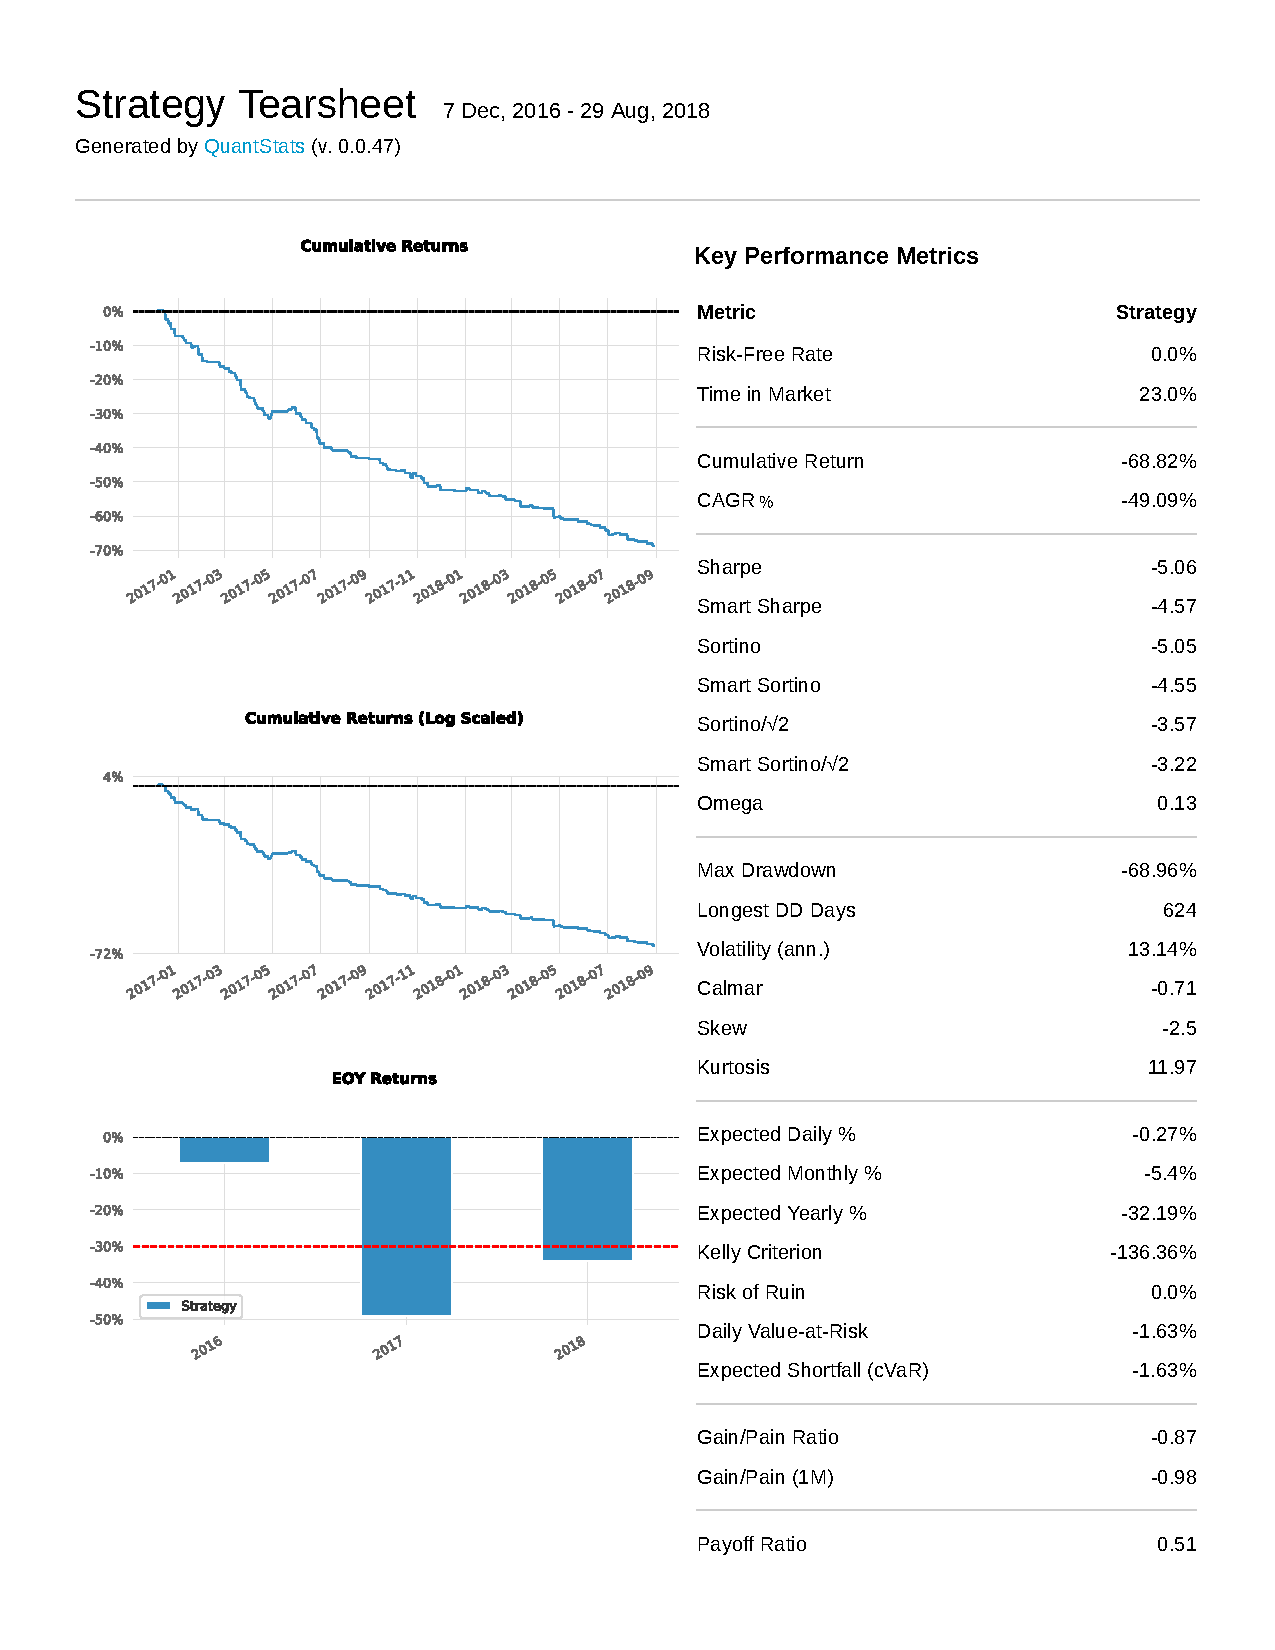
\includegraphics[width=\textwidth]{plots/qs_a2c.pdf}
  \end{subfigure}
  \hspace{0.05\textwidth}
  \begin{subfigure}[ht!]{0.45\textwidth}
    \includegraphics[page=2, width=\textwidth]{plots/qs_a2c.pdf}
  \end{subfigure}
  \begin{subfigure}[ht!]{0.45\textwidth}
    \includegraphics[page=3, width=\textwidth]{plots/qs_a2c.pdf}
  \end{subfigure}
  \caption{Raport Quantstats dla algorytmu A2C na
    danych testowych}
\end{figure}

\begin{figure}[ht!]
  \centering
  \begin{subfigure}[ht!]{0.45\textwidth}
    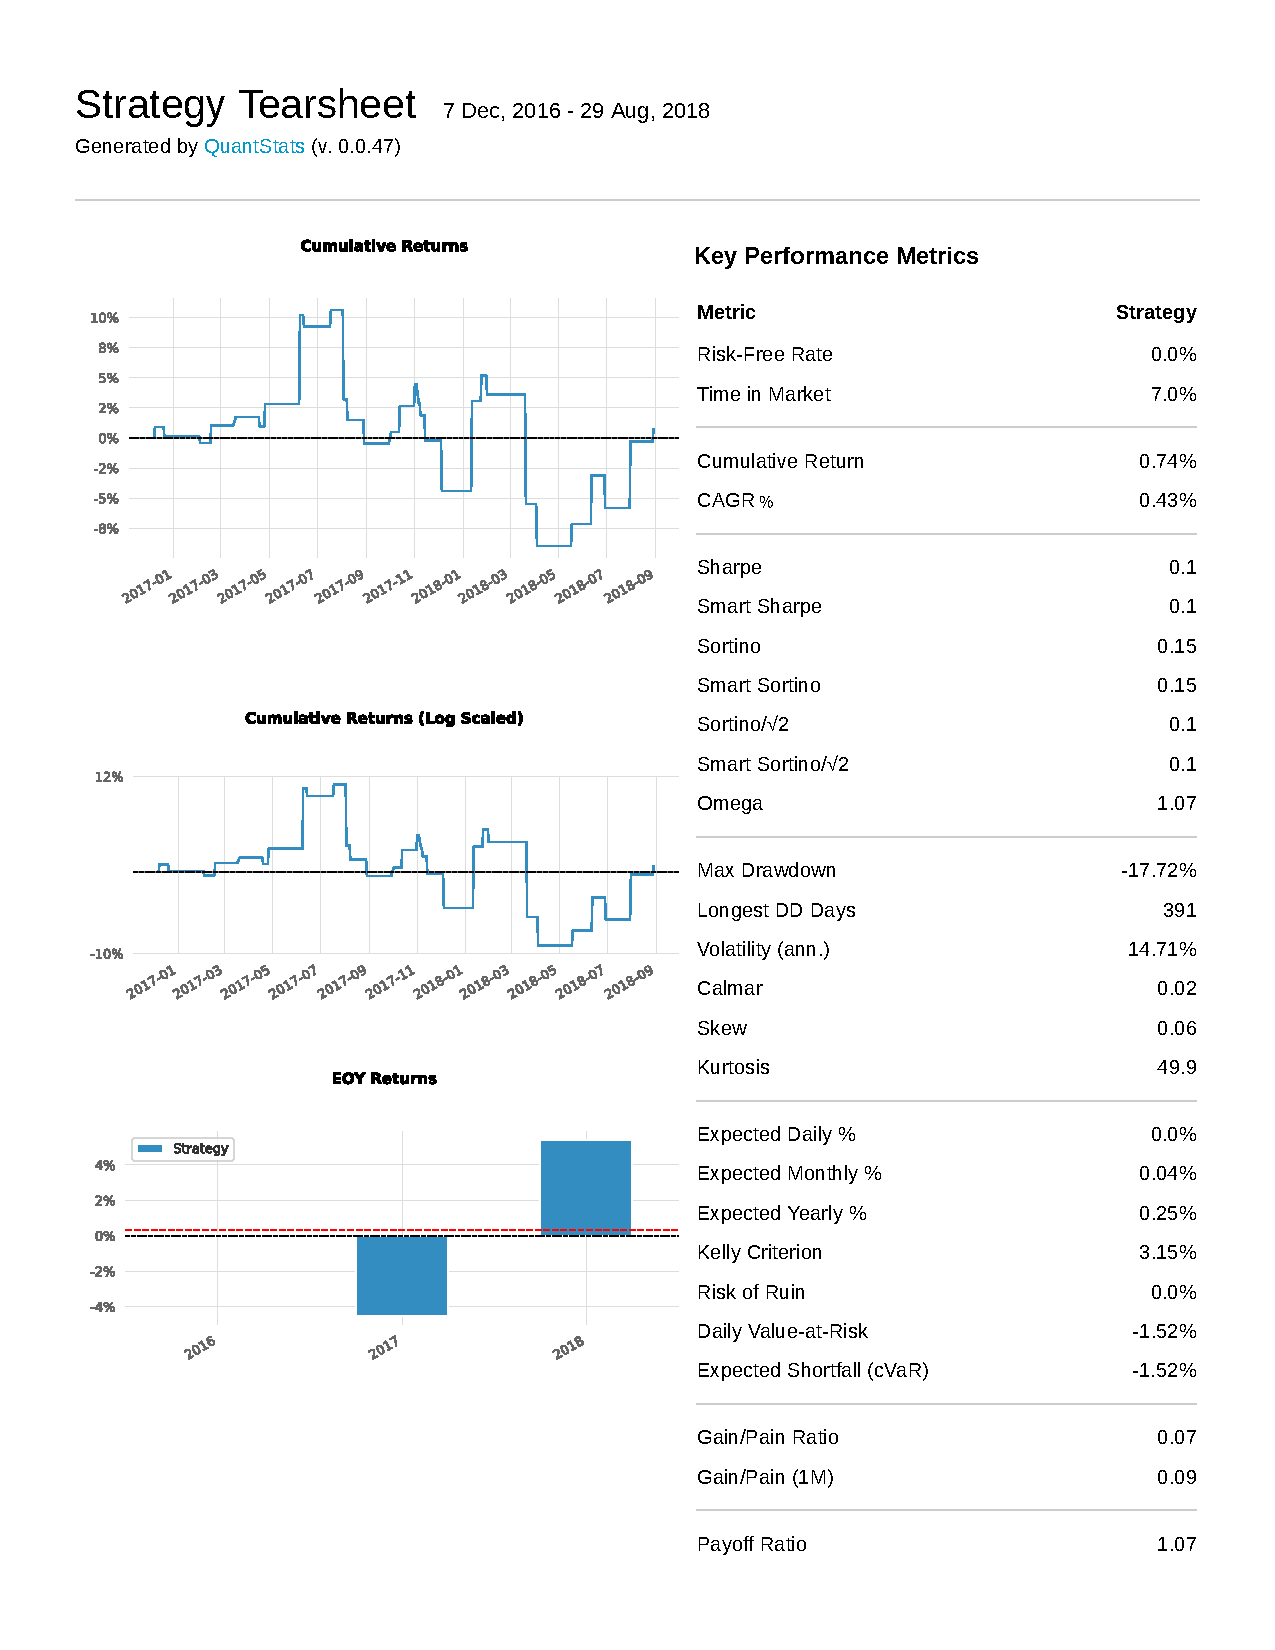
\includegraphics[width=\textwidth]{plots/qs_ppo.pdf}
  \end{subfigure}
  \hspace{0.05\textwidth}
  \begin{subfigure}[ht!]{0.45\textwidth}
    \includegraphics[page=2, width=\textwidth]{plots/qs_ppo.pdf}
  \end{subfigure}
  \begin{subfigure}[ht!]{0.45\textwidth}
    \includegraphics[page=3, width=\textwidth]{plots/qs_ppo.pdf}
  \end{subfigure}
  \caption{Raport Quantstats dla algorytmu PPO na
    danych testowych}
\end{figure}

\begin{figure}[ht!]
  \centering
  \begin{subfigure}[ht!]{0.45\textwidth}
    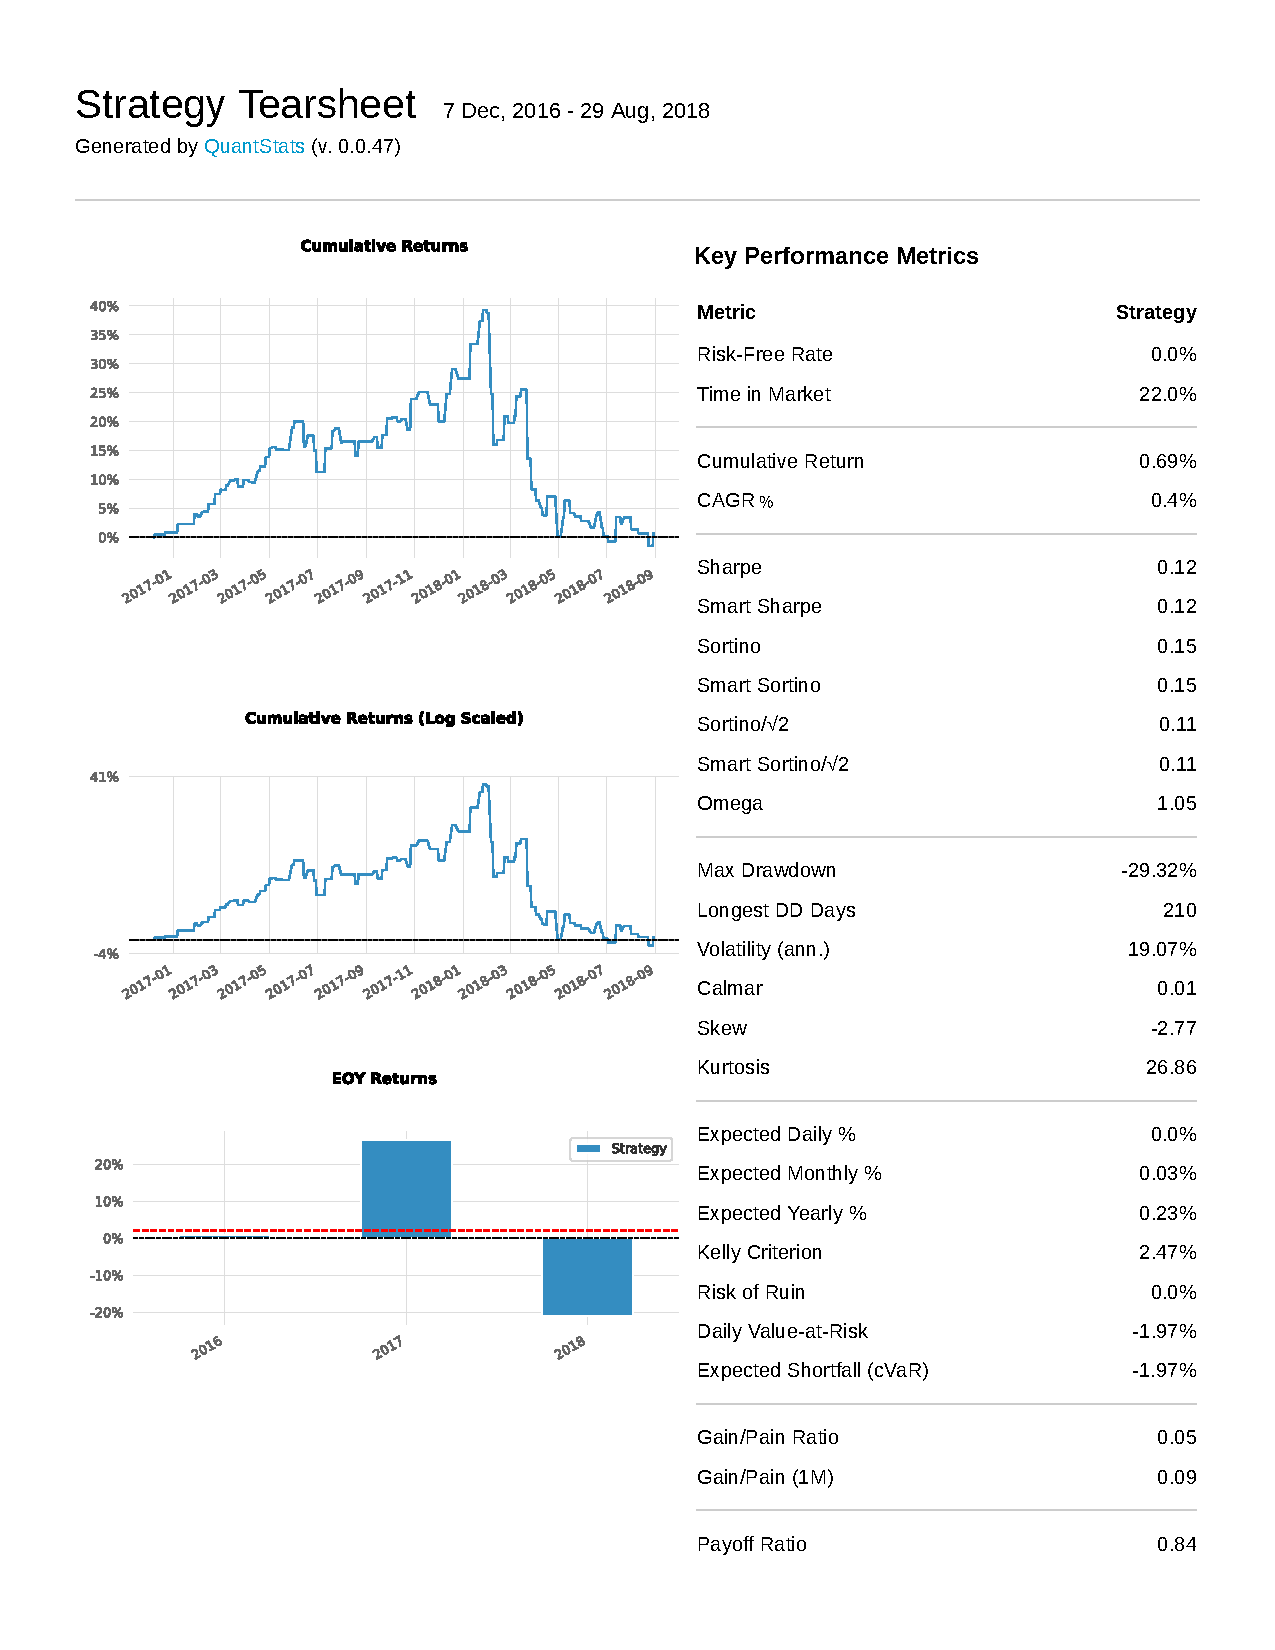
\includegraphics[width=\textwidth]{plots/qs_rppo.pdf}
  \end{subfigure}
  \hspace{0.05\textwidth}
  \begin{subfigure}[ht!]{0.45\textwidth}
    \includegraphics[page=2, width=\textwidth]{plots/qs_rppo.pdf}
  \end{subfigure}
  \begin{subfigure}[ht!]{0.45\textwidth}
    \includegraphics[page=3, width=\textwidth]{plots/qs_rppo.pdf}
  \end{subfigure}
  \caption{Raport Quantstats dla algorytmu RecurrentPPO na
    danych testowych}
\end{figure}

\end{document}
